% !Mode:: "TeX:UTF-8"
\chapter{基于大模型的交通智能体设计}
\section{交通智能体总体架构设计}
本研究设计的交通智能体采用“慢思考（Deliberative Layer）”与“快反应（Reactive Layer）”的双层驱动架构。

慢思考层： 由基于 Qwen-2.5-7B 的大语言模型驱动，负责高层级的用户意图拆解、时空实体提取以及推理逻辑规划。

快反应层： 由一系列预定义的工具链（Tool Chain）组成，包括基础流量查询服务、深度分析引擎以及基于 PDFormer 的流量预测服务。

\begin{figure}[!htbp]
  \centering
  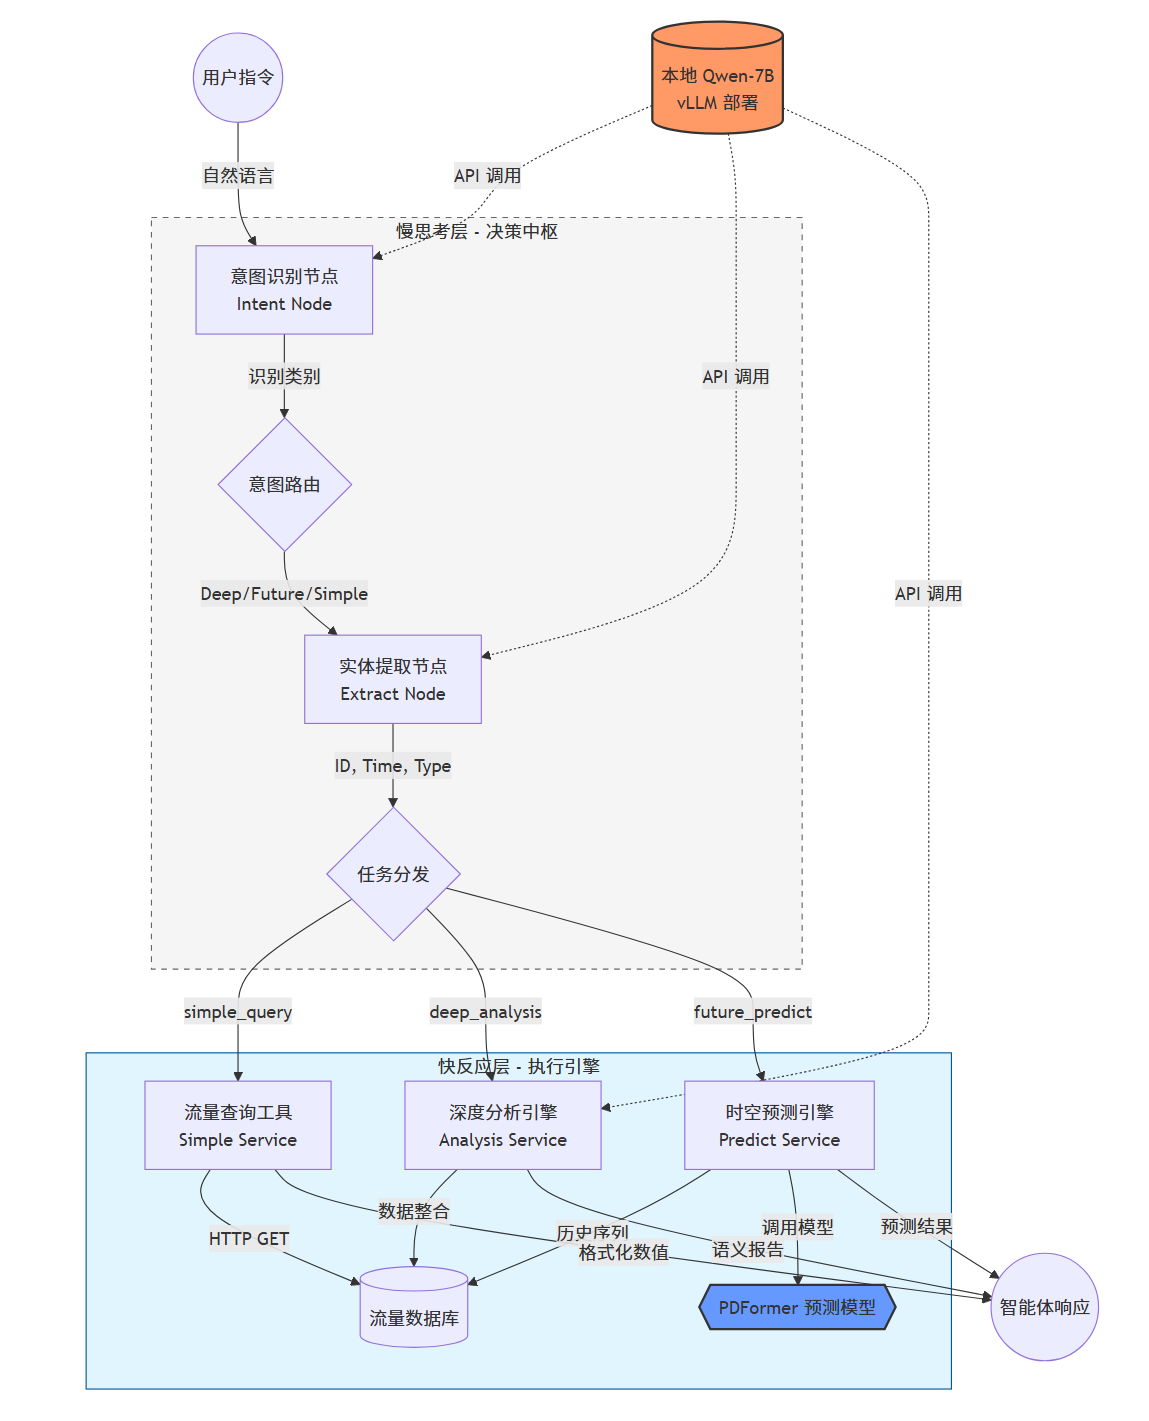
\includegraphics[width=0.7\textwidth]{figure/image4.png}
  \caption{智能体架构设计}
  \label{fig:design}
\end{figure}

本研究的核心推理引擎基于 LangGraph 构建，其本质是将复杂的交通分析任务抽象为一个具备记忆能力的有向无环图（DAG）。与传统的线性 Pipeline 相比，这种架构能够通过显式的状态管理，确保智能体在多步推理中维持极高的时空一致性。每当用户发出一个指令，智能体首先通过意图识别节点（Intent Node）将其分类为数值查询、预测任务或深度分析。随后，时空实体提取节点（Extract Node）会根据预设的提示词模板，从用户输入中抽取出关键的参数，如传感器 ID、时间戳和数据类型，并将这些参数以结构化的格式存储在状态图中。最后，条件路由机制（Conditional Rerouting）根据当前的 WorkflowState 动态选择执行路径，确保智能体能够灵活应对不同类型的请求，同时保持推理过程的连贯性和准确性。

% \vspace{3em}

\section{语言大模型选择与本地化部署}
为了保证交通预测任务的实时性与数据安全性，本研究实现了大语言模型的本地化部署。

基座模型选择： 本研究选用 Qwen-2.5-7B-Instruct 作为智能体的核心决策引擎。该模型基于 Transformer 架构，在预训练阶段采用了超过 18 万亿个 Token 的大规模语料。相比于同参数规模的其他模型，Qwen-2.5 在复杂交通指令的逻辑推理、长文本理解以及多任务分发方面表现出更强的鲁棒性。通过指令微调（Instruction Tuning），该模型能够精准对齐交通工程领域的特定语境，为智能体提供了稳定的符号处理能力。

量化与加速： 针对算力资源优化，采用 GPTQ-Int4 量化方案，显著降低了显存占用，通过将gpu-memory-utilization 设为 0.45 左右，使得 7B 规模的模型能在单张显卡上高效运行，为底层的 PDFormer 模型预留了充足的显存空间，实现了“决策-预测”任务的算力解耦。

推理引擎： 利用 vLLM 推理框架构建满足 OpenAI 协议标准的 API 服务。通过其 PagedAttention 技术，模型能够支持更长的上下文长度，为后续处理多节点、长时间序列的交通特征分析提供了充裕的 Token 空间，在本系统中，我们将最大序列长度（max-model-len）配置为 4096，这使得智能体能够同时感知 7 个传感器节点在过去一个小时内的 84 组特征数据（7 节点 $\times$ 12 步长），并在不截断上下文的前提下，结合历史拓扑关系进行长时程的语义分析与推理。

\vspace{5em}

模型服务启动命令如代码\ref{code-vllm-server}所示。
\begin{lstlisting}[
    language=bash,
    caption={vLLM OpenAI 兼容 API 服务启动命令},
    label={code-vllm-server},
    breaklines=true,
    frame=single,
    numbers=left,
    % 定义用 @ 符号包裹的内容按 LaTeX 原样解析
    escapeinside={@}{@}
]
python -m vllm.entrypoints.openai.api_server \
    --model @\$@MODEL_PATH \
    --served-model-name qwen-7b \
    --host 0.0.0.0 \
    --port 8002 \
    --tensor-parallel-size 1 \
    --gpu-memory-utilization 0.45 \
    --max-model-len 4096 \
    --trust-remote-code \
    --api-key "sk-local-api-key"
\end{lstlisting}

\section{基于状态图的推理逻辑与节点设计}
智能体的核心推理过程被解构为一系列相互协作的逻辑节点：

意图识别节点 (Intent Node)： 利用 LLM 的零样本学习能力，将用户请求归类为数值查询（simple\_query）、预测任务（future\_predict）或深度解读（deep\_analysis），模型的输出被约束在 simple\_query、future\_predict 与 deep\_analysis 三个离散的意图空间内，这种设计有效地防止了模型在复杂交通语境下产生“幻觉”，体现了智能体对交通语义的“慢思考”过程。

时空实体提取节点 (Extract Node)： 由于底层交通流量数据库仅接受严格的数值索引和时间格式，因此采用“完形填空（Infilling）”模式设计的提示词，强制 LLM 将用户口语化的表述转化为标准化的 ID|YYYY-MM-DD HH:MM|Type 字符串，在模型输出后，节点通过正则表达式解析器进行后处理，将文本映射为 Python 内部的 datetime 对象，并生成符合 ISO-8601 标准的时间戳。该节点解决了自然语言与底层数据库索引之间的对齐问题，将非结构化文本转化为机器可执行的参数，为后续工具链的调用提供了精准的输入。

条件路由机制 (Conditional Rerouting)： 系统根据意图标签，将逻辑流导向不同的工具引擎，动态选择执行路径。这种非线性的流转逻辑相比传统的线性 Pipeline，具备更强的异常处理能力，显著增强了系统在面对复杂交通任务时的可扩展性。

\section{执行层工具链设计与实现}
在本项目设计的执行层中，各核心工具被封装为基于 FastAPI 异步框架的微服务节点，从而实现了交通智能体与物理世界数据之间的动态感知与交互。该层级通过 Uvicorn 高性能服务器进行部署，将存储于 SQLite 数据库中的静态交通原子文件转化为可实时调用的计算资源。

在基础流量感知维度上，系统实现了流量感知工具的交互接口。该工具通过 /flow/point 端点接收来自智能体的实体标识与 ISO-8601 格式的时间参数，并在后端利用 SQL 语句的模式匹配机制对 dyna 动态表进行毫秒级的检索。为了确保数据提取的精确性与工程鲁棒性，该服务在底层数据库连接中采用了 sqlite3.Row 工厂模式，这使得原始的机动车、非机动车及行人流量数值能够以高度结构化的键值对形式反馈至智能体状态图中。这种设计不仅解决了时空数据在跨模块传递过程中的格式对齐问题，更为智能体提供了瞬时态势感知的物理基础。

针对更高层级的决策需求，本研究进一步设计了深度分析节点作为数据支撑。该引擎的核心逻辑在于其对历史流量序列的动态回溯能力，通过 /flow/history 接口实现。服务端利用 Python 的 datetime 类与 timedelta 偏移逻辑，根据智能体下发的查询跨度参数自动计算时空起止坐标，并从数据库中提取具有连续性的流量序列。为了提升智能体在处理长序列数据时的效率，该分析引擎在返回结果前会执行初步的特征聚合，仅保留流量波动的关键时间节点，从而支撑智能体利用链式思考机制对当前路段的拥堵风险或人车干扰程度生成具有专家水准的评估报告。

在预测任务的执行过程中，预测计算工具（Predict Service）作为智能体与底层 PDFormer 时空模型的集成中枢发挥了关键作用。该工具不再局限于单点的数值检索，而是通过在全网 7 个传感器节点上同步采集过去 12 个历史步长的全局特征，构建出完备的时序特征向量。这种基于 FastAPI 的微服务化设计实现了“感知逻辑”与“数值计算”在工程层面的完全解耦。智能体仅需通过标准的 HTTP 协议发送 JSON 格式的数据包，即可触发位于特定端口的预测引擎运行复杂的时空变换算法。预测结果最终以对齐格式的表格形式输出，实现了数值、语义与图表的多维度信息反馈。系统还集成了基于文件处理器的日志审计模块，对每一次 API 调用进行实时记录，为系统在复杂交通场景下的稳健运行提供了底层的工程保障。
